%!TEX root = thesis.tex

\chapter{Grundlagen} % (fold)
\label{cha:grundlagen}

Grundlagen mit den bisherigen Quellen \citealt{play_for_scala_v8}.

In diesem Kapitel werden die grundlegenden Techniken zur Webseiten-Entwicklung mit dem Play-Framework vorgestellt werden.
Dabei wird dafür benötigtes Hintergrundwissen bereitgestellt und erklärt, welche Werkzeuge benötigt werden.
Schließlich werden durch die Entwicklung einer kleinen Anwendung die einzelnen Komponenten erklärt.
Es werden hierbei in erster Linie die Komponenten vorgestellt, die für die Entwicklung von Real-Time-Web-Anwendungen unbedingt notwendig sind.


\section{Vorbereitung} % (fold)
\label{sec:vorbereitung}

Bevor auf die eigentliche Arbeit mit dem Play-Framework eingegangen wird, müssen einige vorbereitende Dinge geklärt werden. In diesem Abschnitt geht es darum, wie die Entwicklungsumgebung aufgesetzt wird, mit welcher Version der eingesetzten Software gearbeitet wird und wie sich das Play-Framework installieren lässt.

\subsection{Entwicklungsumgebung} % (fold)
\label{sub:entwicklungsumgebung}

Zum Anlegen von Play-Projekten und Steuern des Web-Servers wird eine Kommandozeile, wie die Eingabeaufforderung unter Windows oder dem Terminal und Mac OS~X benötigt.
Zum Programmieren kann entweder ein einfacher Text-Editor, oder auch eine \gls{ide} verwendet werden.
Für die einzelnen Programme können teilweise Plugins heruntergeladen werden, die beispielsweise code completion oder syntax highlighting für Play-spezifische Funktionalitäten bereitstellen.

Für \textbf{Eclipse} kann die Scala IDE von \citealt{scala_ide} heruntergeladen werden.
Diese IDE ist für die Entwicklung von Scala-Anwendungen mit Eclipse notwendig.
Für die Scala IDE existiert außerdem ein Plugin für das Play-Framework.
Eine genaue Installationsanleitung dafür ist unter \citealt{scala_ide_play_plugin} zu finden.
Um ein Play-Projekt in Eclipse zu bearbeiten, muss dafür nach dem Anlegen des Projekts auf der Kommandozeile ein Eclipse-Projekt exportiert werden.
Dazu muss in der Play-Konsole des Projekts der Befehl \lstinline|eclipse| ausgeführt werden.
Dieser Befehl muss jedes Mal ausgeführt werden, wenn die Konfigurationsdateien geändert werden.
Anschließend kann der Ordner des Play-Projekts als Eclipse-Projekt importiert und geöffnet werden.

Beim Exportieren eines \textbf{IntelliJ IDEA}-Projekts verhält es sich ähnlich, wie im Falle von Eclipse.
Der einzige Unterschied ist, dass der Befehel \lstinline|idea| verwendet werden muss, um ein IntelliJ IDEA-Projekt zu erstellen.
Für Text-Editoren, wie z.B. \textbf{VIM}, \textbf{Emacs} oder \textbf{Sublime Text} ist prinzipiell kein Plugin nötig, es kann aber eines installiert werden, sofern eines vorhanden ist.
Weitere Informationen zu diesen und \textbf{anderen Entwicklungsumgebungen} sind in der offiziellen Dokumentation zu finden \cite[vgl.][]{ide}.

% subsection entwicklungsumgebung (end)


\subsection{Software-Version} % (fold)
\label{sub:software_version}

Zum Zeitpunkt dieser Arbeit ist die aktuellste stabile Version des Play-Frameworks die Version 2.1.2.
Diese Version wird in allen Beispielen und der eigenen entwickelten Anwendung verwendet.
Für den Einsatz des Frameworks wird das JDK (Java development kit) in Version 6 oder 7 benötigt.
Der Autor arbeitet mit dem JDK~7 unter Mac OS~X.

% subsection software_version (end)


\subsection{Installation} % (fold)
\label{sub:installation}

Zum Installieren von Play kann eine vorkompilierte Version der Software von der offiziellen Website unter \cite{play_download} heruntergeladen werden.
Nach dem Entpacken der heruntergeladenen Datei kann das Programm namens \lstinline|play|, das sich im entpackten Ordner befindet, auf der Kommandozeile verwendet werden.
Um für die Verwendung des Programms nicht immer den absoluten Pfad angeben zu müssen, kann der Pfad zum entpackten Ordner in die Systemumgebungsvariable PATH eingetragen werden.

Unter \textbf{Mac OS~X} muss dazu auf der Kommandozeile folgender Befehl ausgeführt werden: \lstinline|export PATH=$PATH:<Pfad zum entpackten Ordner>|.
Ein konkretes Beispiel könnte so aussehen: \lstinline|export PATH=$PATH:~/Downloads/play-2.1.2|.
Damit sich der Ordner auch nach dem Schließen des Terminals noch in der PATH-Variable befindet, sollte der obige Befehl zusätzlich in die \lstinline|~/.profile|-Datei eingetragen werden.
Falls diese Datei nicht existiert, muss sie vorher angelegt werden.

Unter \textbf{Windows} muss dazu in der Eingabeaufforderung folgender Befehl ausgeführt werden: \lstinline|setx PATH "%PATH%;c:\path\to\play" /m|, wobei \lstinline|c:\path\to\play| durch den tatsächlichen Pfad zu ersetzen ist \cite[vgl.][S.~9]{play_for_scala_v8}.

% subsection installation (end)


\section{Architektur} % (fold)
\label{sec:architektur}

Auf der untersten Ebene existiert ein Web-Server, der mit dem Framework ausgeliefert wird.
Die Anfragen, die der Web-Server empfängt werden an Play weitergeleitet und schließlich von der Anwendung verarbeitet.
Nach der Verarbeitung wird eine Antwort generiert und schließlich als HTTP-Antwort versendet.
Der Anwendungscode einer Play-Applikation ist nach der \gls{mvc}-Architektur aufgebaut \cite[vgl.][S.~51-53]{play_for_scala_v8}.

"`[\gls{mvc} programming is a] three-way factoring, whereby objects of different classes take over the operations related to the application domain (the model), the display of the application's state (the view), and the user interaction with the model and the view (the controller)."' \cite[vgl.][S.~1]{mvc}.
Views bilden Models i.~d.~R. auf HTML-Seiten ab.
Controller sind dazu da, HTTP-Anfragen zu verarbeiten, die jeweilige Antwort durch eine View übersetzen zu lassen und als HTTP-Antwort zurückzusenden.

% section architektur (end)


% section vorbereitung (end)


\section{Erstellen einer Anwendung} % (fold)
\label{sec:erstellen_einer_anwendung}

Um eine neue Anwendung mit Play zu erstellen, muss auf der Kommandozeile in den Ordner navigiert werden, in dem das Projekt erstellt werden soll.
Anschließend kann mit \lstinline[language=sh]|play new <project name>| ein neues Projekt angelegt werden.
Im startenden Assistenten wählt man die Hauptprogrammiersprache aus (Java oder Scala), in diesem Fall Scala.
Daraufhin wird im aktuellen Verzeichnis ein neuer Ordner mit dem vorher angegebenen Namen \lstinline|<project name>| angelegt \cite[vgl.][S.~10]{play_for_scala_v8}.
Die darin vorzufindende Verzeichnisstruktur wird im nächsten Abschnitt beschrieben.

% section erstellen_einer_anwendung (end)


\section{Verzeichnisstruktur} % (fold)
\label{sec:verzeichnisstruktur}

Die Verzeichnisstruktur einer Play-Anwendung ist immer gleich.
An dieser Stelle werden nur die Ordner vorgestellt, die für das Verständnis dieser Arbeit wichtig sind.
Diese Ordner sind folgende \cite[vgl.][]{play_verzeichnisstruktur}:

\begin{description}[leftmargin=!,labelwidth=\widthof{\bfseries app/controllers/}]
  \item[app/] ausführbare Komponenten
  \item[app/controllers/] Controller-Komponenten
  \item[app/models/] Model-Komponenten
  \item[app/views/] View-Komponenten
  \item[conf/] Konfigurationsdateien
  \item[public/] öffentliche statische Dateien (\gls{js}, \gls{css}, Bilder)
\end{description}

% section verzeichnisstruktur (end)


\section{Starten einer Anwendung} % (fold)
\label{sec:starten_einer_anwendung}

Um die neu erstellte Anwendung zu starten, muss sie erst kompiliert werden.
Das geschieht ebenfalls mit Hilfe des \lstinline|play|-Befehls.
Mit dem Aufruf von \lstinline|play| gelangt man in die Play-Konsole.
Von dort aus kann mit \lstinline|compile| der Source-Code kompiliert und anschließend mit \lstinline|run| ausgeführt werden.
Der Aufruf von \lstinline|compile| ist allerdings optional.
Falls noch nicht kompilierte Änderungen existieren, werden diese beim Aufruf von \lstinline|run| automatisch kompiliert, sobald die Website aufgerufen wird \cite[vgl.][]{play_compile}.

Jede neue Play-Anwendung ist eine lauffähige Website.
Diese kann nach dem Starten unter der URL \url{http://localhost:9000/} abgerufen werden (siehe Abb.~\ref{fig:anwendung_nach_erstellung}).
Um die Anwendung bei Dateiänderungen automatisch neu kompilieren zu lassen, ohne sie erst im Browser aufrufen zu müssen, kann in der Play-Konsole statt \lstinline|run| \lstinline|~run| ausgeführt werden \cite[vgl.][S.~12--13]{play_for_scala_v8}.

\begin{figure}[h]
\centering
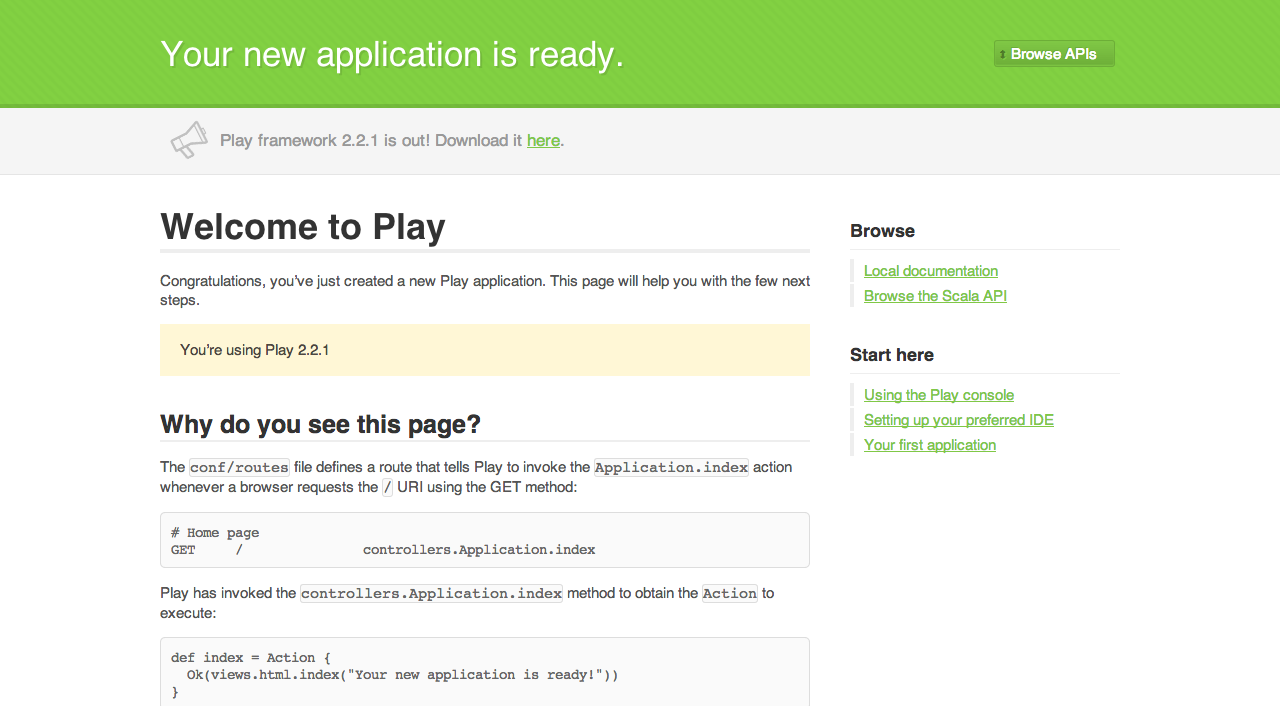
\includegraphics[width=\textwidth]{hello_world.png}
\caption{Eine neu erstellte Play-Anwendung}
\label{fig:anwendung_nach_erstellung}
\end{figure}

% section starten_einer_anwendung (end)


\section{Beispielanwendung: Sammeln von Altersstatistiken} % (fold)
\label{sec:beispielanwendung}

Um die Techniken zur Entwicklung von statischen Web-Anwendungen zu demonstrieren, soll im Folgenden eine kleine Anwendung entwickelt werden.
Diese Anwendung fragt ihre Benutzer, wie alt sie sind und bildet die gesammelten Information als Diagramm ab.
Anhand dieser Anwendung soll die Entwicklung mit Models, Views und Controllern erklärt werden.


\subsection{Routing} % (fold)
\label{sub:routing}

Wenn die Website von jemandem aufgerufen wird, soll eine bestimmte Controller-Aktion ausgeführt werden.
Damit Play weiß, welche Controller-Aktion für die aufgerufene URL ausgeführt werden soll, muss dies im \gls{router} definiert werden.
Der Router befindet sich unter \lstinline|conf/routes| und besitzt nach der Erstellung einer Anwendung bereits zwei Einträge (vgl. Listing~\ref{lst:der_router}).
An dieser Stelle ist allerdings nur der erste Eintrag interessant.

\begin{lstlisting}[caption=Der Router, label=lst:der_router]
  GET    /    controllers.Application.index
\end{lstlisting}

Dieser Eintrag bedeutet, dass HTTP-Anfragen der Methode \lstinline|GET| der URL \lstinline|/| auf die Controller-Aktion \lstinline|index| des Controllers \lstinline[breaklines=true]|controllers.Application| abgebildet werden.
Neben \lstinline|GET| gibt es noch \lstinline|POST|, \lstinline|PUT|, \lstinline|DELETE| und \lstinline|HEAD|.
Die am Häufigsten verwendeten HTTP-Methoden sind \lstinline|GET|, \lstinline|POST|, \lstinline|PUT| und \lstinline|DELETE|, um Daten abzufragen, zu bearbeiten, zu erstellen und zu löschen \cite[vgl.][S.~6]{play_for_scala_v8}.
Der Pfad \lstinline|/| steht für die URL \url{http://localhost:9000/}.
Es sind auch längere Pfade, wie z.~B. \lstinline|/animals/cat| möglich, davon wird in diesem Beispiel allerdings nicht Gebrauch gemacht.
Die Controller-Aktion \lstinline|controllers.Application.index|, auf die der Routing-Eintrag zeigt, ist bereits implementiert. Diese wird im nächsten Abschnitt näher erläutert.

% subsection routing (end)


\subsubsection{Controller} % (fold)
\label{ssub:controller}

Nachdem im Router definiert wurde, welche URLs auf welche Controller-Aktionen abgebildet werden sollen, werden nun die dazugehörigen Controller-Aktionen erklärt.
Die zuvor genannte Aktion \lstinline[breaklines=true]|controllers.Application.index| befindet sich in der Datei \lstinline[breaklines=true]|app/controllers/Application.scala| und ist, wie in Listing~\ref{lst:application_controller_mit_index_aktion} zu sehen, definiert.

\begin{lstlisting}[caption=Der Application-Controller mit index-Aktion, label=lst:application_controller_mit_index_aktion]
object Application extends Controller {
  def index = Action {
    Ok(views.html.index("Your new application is ready."))
  }
}
\end{lstlisting}

Controller sind Objekte, die von \lstinline|Controller| erben und Aktionen definieren.
Aktionen, die beim Aufruf einer URL ausgeführt werden sollen, sind Controller-Objekt-Methoden mit dem Rückgabetyp \lstinline|Action|.
Eine Aktion, bzw. \lstinline|Action| ist eine Funktion von einer HTTP-Anfrage nach einer HTTP-Antwort.
In der obigen Form wird die HTTP-Anfrage ignoriert, es können aber auch \lstinline|Action|s mit explizitem oder implizitem Request erstellt werden \cite[vgl.][]{play_controllers}.
Das könnte aussehen, wie in Listing~\ref{lst:action_mit_implizitem_request} gezeigt.

\begin{lstlisting}[caption=Action mit implizitem Request, label=lst:action_mit_implizitem_request]
def index = Action { implicit request =>
  Ok(views.html.index("Your new application is ready."))
}
\end{lstlisting}

Um eine HTTP-Antwort zu generieren, stellt das Objekt \lstinline|play.api.mvc.Results|, von dem \lstinline|play.api.mvc.Controller| erbt, mehrere Konstruktoren zur Verfügung.
Der in Listing~\ref{lst:application_controller_mit_index_aktion} und \ref{lst:action_mit_implizitem_request} verwendete Konstruktor \lstinline|Ok| erstellt eine HTTP-Antwort mit dem Status-Code \lstinline|200 OK|.
Der Inhalt dieser Antwort ist das Ergebnis der View \lstinline|views.html.index|, worauf im folgenden Abschnitt näher eingegangen wird.
Neben \lstinline|Ok| gibt es u.~a. noch \lstinline|BadRequest| für fehlerhafte Anfragen (z.~B. unvollständiges Formular) und \lstinline|Redirect|, um eine Seitenweiterleitung auf eine angegebene URL durchzuführen \cite[vgl.][]{play_controllers}.

% subsubsection controller (end)


\subsection{View} % (fold)
\label{sub:view}

Im vorigen Abschnitt wurde gezeigt, wie mittels \lstinline[breaklines=true]|Ok(views.html.index("Your new application is ready."))| eine View gerendert und als HTTP-Antwort verschickt wurde.
Das View-Template befindet sich unter \lstinline|app/views/index.scala.html| und hat den in Listing~\ref{lst:das_index_view_template} gezeigten Inhalt.

\begin{lstlisting}[caption=Das index-View-Template, label=lst:das_index_view_template]
@(message: String)

@main("Welcome to Play 2.1") {
    @play20.welcome(message)
}
\end{lstlisting}

View-Templates bestehen aus Scala- und HTML-Code.
Am Anfang eines Templates steht die Parameterliste, worüber die anzuzeigenden Daten übergeben werden.
Das \lstinline|@|-Symbol führt einen Scala-Ausdruck an.
Andere View-Templates und sog. Helper können wie normale Funktionen aufgerufen werden.
Helper sind in Funktionen ausgelagerter View-Code.
\lstinline|@play20.welcome(message)| ist ein Aufruf eines solchen Helpers, der die in Abb.~\ref{fig:anwendung_nach_erstellung} abgebildete Seite generiert.
\lstinline|@main("Welcome to Play 2.1") { /* ... */ }| ist ein Aufruf eines anderen Templates.
Dieses Template ist unter \lstinline|app/views/main.scala.html| zu finden und generiert das Grundgerüst der Website aus dem Webseiten-Titel (der ersten Parameterliste) und dem eigentlichen Inhalt (der zweiten Parameterliste).
In diesem Template werden durch  Aufrufe wie \lstinline[breaklines=true]|@routes.Assets.at("javascripts/jquery-1.9.0.min.js")| Dateien aus dem \lstinline|public/|-Ordner adressiert.

% subsection view (end)


% section beispielanwendung (end)


% chapter grundlagen (end)